\documentclass[aspectratio=169]{beamer}

\usepackage{ccicons}
\usepackage{fontspec}
\usepackage{import}
\usepackage{listings}
\usepackage{tikz}

\subimport{../}{colors.tex}

\usetikzlibrary{
  arrows,
  arrows.meta,
  automata,
  backgrounds,
  calc,
  chains,
  decorations.pathreplacing,
  fit,
  matrix,
  overlay-beamer-styles,
  positioning,
  shapes,
  tikzmark,
}
\usetikzmarklibrary{listings}

\hypersetup{
  colorlinks=true,
  urlcolor=uclablue,
}

\setbeamercolor{frametitle}{fg=primarycolor}
\setbeamercolor{structure}{fg=primarycolor}
\setbeamercolor{enumerate item}{fg=black}
\setbeamercolor{itemize item}{fg=black}
\setbeamercolor{itemize subitem}{fg=black}

\setbeamersize{text margin left=26.6mm}
\addtolength{\headsep}{2mm}

\setbeamertemplate{navigation symbols}{}
\setbeamertemplate{headline}{}
\setbeamertemplate{footline}{}
\setbeamertemplate{itemize item}{\color{black}}
\setbeamertemplate{itemize items}[circle]

\setbeamertemplate{footline}{
  \begin{tikzpicture}[remember picture,
                      overlay,
                      shift={(current page.south west)}]
    \node [black!50, inner sep=2mm, anchor=south east]
          at (current page.south east) {\footnotesize \insertframenumber};
  \end{tikzpicture}
}

\setsansfont{Overpass}[Scale=MatchLowercase]
\setmonofont{Overpass Mono}[Scale=MatchLowercase]

\makeatletter
\newcommand\version[1]{\renewcommand\@version{#1}}
\newcommand\@version{}
\def\insertversion{\@version}

\newcommand\lecturenumber[1]{\renewcommand\@lecturenumber{#1}}
\newcommand\@lecturenumber{}
\def\insertlecturenumber{\@lecturenumber}
\makeatother

\setbeamertemplate{title page}
{
  \begin{tikzpicture}[remember picture,
                      overlay,
                      shift={(current page.south west)},
                      background rectangle/.style={fill=uclablue},
                      show background rectangle]
    \node [anchor=west, align=left, inner sep=0, text=white]
          (lecturenumber) at (\paperwidth / 6, \paperheight * 3 / 4)
          {\Large Lecture \insertlecturenumber};
    \node [inner sep=0, align=left, text=white, node distance=0,
           above left=of lecturenumber, anchor=south west, yshift=2mm]
          {\Large CS 111: Operating System Principles};
    \node (title) [inner sep=0, anchor=west, align=right, text=white]
          at (\paperwidth / 6, \paperheight / 2)
          {{\bfseries \Huge \inserttitle{}}};
    \node [inner sep=0, align=right, text=white, node distance=0,
           below right=of title, anchor=north east, yshift=-1mm]
          {{\footnotesize \ttfamily \insertversion}};
    \node [inner sep=0, text=white, align=left, anchor=west]
          (author) at (\paperwidth / 6, \paperheight / 4)
          {\insertauthor};
    \node [text=white, inner sep=0, align=left, node distance=0,
           below left=of author, anchor=north west, yshift=-2mm]
          {\insertdate};
    \node [align=right, anchor=south east, inner sep=2mm, text=white]
          (license) at (\paperwidth, 0)
          {\footnotesize This  work is licensed under a
           \href{http://creativecommons.org/licenses/by-sa/4.0/}
                {\color{uclagold} Creative Commons Attribution-ShareAlike 4.0
                 International License}};
    \node [text=white, inner sep=0, align=right, node distance=0,
           above right=of license, anchor=south east, xshift=-2mm]
          {\Large \ccbysa};
  \end{tikzpicture}
}

\tikzset{
  >=Straight Barb[],
  shorten >=1pt,
  initial text=,
}

\lstset{
  basicstyle=\footnotesize\ttfamily,
}


\lecturenumber{4}
\title{Processes}
\version{2.0.0}
\author{Jon Eyolfson}
\date{July 1, 2021}

\begin{document}
  \begin{frame}[plain, noframenumbering]
    \titlepage
  \end{frame}

  \begin{frame}
    \frametitle{A Process is an Instance of a Running Program}

    A program (or application) is just a static definition, including:

    \begin{itemize}
      \item Instructions
      \item Data
      \item Memory allocations
      \item Symbols it uses
    \end{itemize}

    \vspace{2em}

    When you start executing a program, it turns into a process
  \end{frame}

  \begin{frame}
    \frametitle{Process is like a Combination of all the Virtual Resources}

    If we consider a ``virtual CPU'', the OS needs to track all registers

    \vspace{2em}

    It also contains all other resources it can access (memory and I/O)

    \vspace{4em}

    Every execution runs the same code (part of the program)

    \hspace{2em} An execution is running some specific code (part of the
                 process)
  \end{frame}

  \begin{frame}
    \frametitle{A Process is More Flexible}

    A process contains both the program and information specific
    to its execution

    \vspace{4em}

    It allows multiple executions of the same program

    \vspace{2em}

    It even allows a process to run multiple copies of itself
  \end{frame}

  \begin{frame}
    \frametitle{A Process Control Block (PCB) Contains All Execution Information}


    Specifically, in Linux, this is the \texttt{\color{primarycolor}
    task\_struct} saw in Lab 0

    \vspace{2em}

    It contains:
    \begin{itemize}
      \item Process state
      \item CPU registers
      \item Scheduling information
      \item Memory management information
      \item I/O status information
      \item Any other type of accounting information
    \end{itemize}
  \end{frame}

  \begin{frame}
    \frametitle{Aside: Concurrency and Parallelism Aren't the Same}

    Concurrency

    \hspace{2em} Switching between two or more things (can you get interrupted)

    \hspace{4em} Goal: make progress on multiple things

    \vspace{4em}

    Parallelism

    \hspace{2em} Running two or more things at the same time (are they independent)

    \hspace{4em} Goal: run as fast as possible
  \end{frame}

  \begin{frame}
    \frametitle{A Real Life Situation of Concurrency and Parallelism}


    You're sitting at a table for dinner, and you can:
    \begin{itemize}
      \item Eat
      \item Drink
      \item Talk
      \item Gesture
    \end{itemize}
    You're so hungry that if you start eating you won't stop until you finish

    \vspace{4em}

    Which tasks can and can't be done concurrently, and in parallel?
  \end{frame}

  \begin{frame}
    \frametitle{Choose Any Two Tasks in the Real Life Example}

    You can't eat and talk (or drink) at the same time, and you can't switch

    \hspace{2em} Not parallel and not concurrent

    \vspace{2em}

    You could eat and gesture at the same time, but you can't switch

    \hspace{2em} Parallel and not concurrent

    \vspace{2em}

    You can't drink and talk at the same time, and you could switch

    \hspace{2em} Not parallel and concurrent

    \vspace{2em}

    You can talk (or drink) and gesture at the same time, and you could switch

    \hspace{2em} Parallel and concurrent
  \end{frame}


  \begin{frame}
    \frametitle{Uniprogramming is for Old Batch Processing Operating Systems}

    Uniprogramming: only one process running at a time

    \hspace{2em} Two processes are not parallel and not concurrent, no matter what

    \vspace{2em}

    Multiprogramming: allow multiple processes

    \hspace{2em} Two processes can run in parallel or concurrently

    \vspace{4em}

    Modern operating systems try to run everything in parallel and concurrently
  \end{frame}

  \begin{frame}
    \frametitle{Process State Diagram (You Could Rename Waiting to Ready)}

    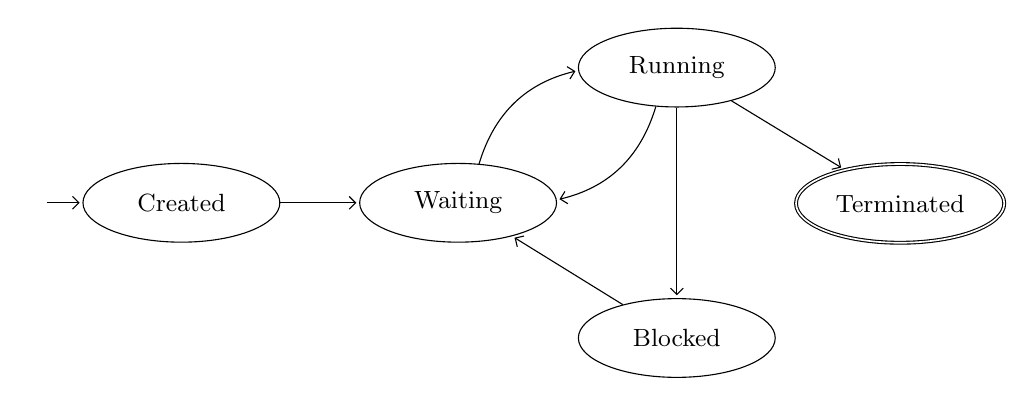
\begin{tikzpicture}[
      every state/.style={ellipse, minimum width=2.5cm, minimum height=1cm, font=\small},
    ]
      \node [state, initial] (created) {Created};
      \node [state, right=of created] (waiting) {Waiting};
      \node [state, above right=of waiting] (running) {Running};
      \node [state, below right=of waiting] (blocked) {Blocked};
      \node [state, accepting, below right=of running] (terminated) {Terminated};
      \path [->] (created) edge (waiting)
                 (waiting) edge [bend left] (running)
                 (running) edge [bend left] (waiting)
                 (running) edge (blocked)
                 (blocked) edge (waiting)
                 (running) edge (terminated);
    \end{tikzpicture}
  \end{frame}

  \begin{frame}
    \frametitle{The Scheduler Decides When To Switch}

    To create a process, the operating system has to at least load it into memory

    \hspace{2em}

    When it's waiting, the scheduler (coming later) decides when it's running

    \hspace{2em}

    We're going to first focus on the mechanics of switching processes
  \end{frame}

  \begin{frame}
    \frametitle{The Core Scheduling Loop Changes Running Processes}

    \begin{enumerate}
      \item Pause the currently running process 
      \item Save its state, so you can restore it later
      \item Get the next process to run from the scheduler
      \item Load the next process' state and let that run
    \end{enumerate}
  \end{frame}

  \begin{frame}
    \frametitle{We Can Let Processes Themselves, or the Operating System Pause}
    
    Cooperative multitasking

    \hspace{2em} The processes use a system call to tell the operating system to
    pause it

    \vspace{2em}

    True multitasking

    \hspace{2em} The operating system retains control and pauses processes

    \vspace{4em}

    For true multitasking the operating system can:

    \begin{itemize}
      \item Give processes set time slices
      \item Wake up periodically using interrupts to do scheduling
    \end{itemize}
  \end{frame}

  \begin{frame}
    \frametitle{Swapping Processes is called Context Switching}

    We've said that at minimum we'd have to save all of the current registers

    \hspace{2em} We have to save all of the values, using the same CPU as we're
    trying to save

    \vspace{2em}

    There's hardware support for saving state, however you may not want to save
    everything

    \vspace{2em}

    Context switching is pure overhead, we want it to be as fast as possible


    \vspace{4em}

    Usually there's a combination of hardware and software to save as little as
    possible
  \end{frame}

  \begin{frame}
    \frametitle{We Could Create Processes from Scratch}

    We load the program into memory and create the process control block

    \vspace{2em}

    This is what Windows does

    \vspace{4em}

    Could we decompose this into more flexible abstractions?
  \end{frame}

  \begin{frame}
    \frametitle{Instead of Creating a New Process, We Could Clone It}

    Pause the currently running process, and copy it's PCB into a new one

    \hspace{2em} This will reuse all of the information from the process,
    including variables!

    \vspace{2em}

    Distinguish between the two processes with a parent and child relationship

    \hspace{2em} They could both execute different parts of the program together

    \vspace{4em}

    We could then allow either process to load a new program and setup a new PCB
  \end{frame}

  \begin{frame}
    \frametitle{On Unix, the Kernel Launches A Single User Process}

    After the kernel initializes, it creates a single process
    from a program

    \vspace{2em}

    This process is called \texttt{init}, and it looks for it in \texttt{/sbin/init}

    \hspace{2em} Responsible for executing every other process on the machine

    \hspace{2em} Must always be active, if it exits the kernel thinks you're shutting down

    \vspace{2em}

    For Linux, \texttt{init} will probably be \texttt{systemd} but there's other options

    \vspace{2em}

    Aside: some operating systems create an ``idle'' process that the
    scheduler can run
  \end{frame}

  \begin{frame}
    \frametitle{A Typical Process Tree on the Virtual Machine}

    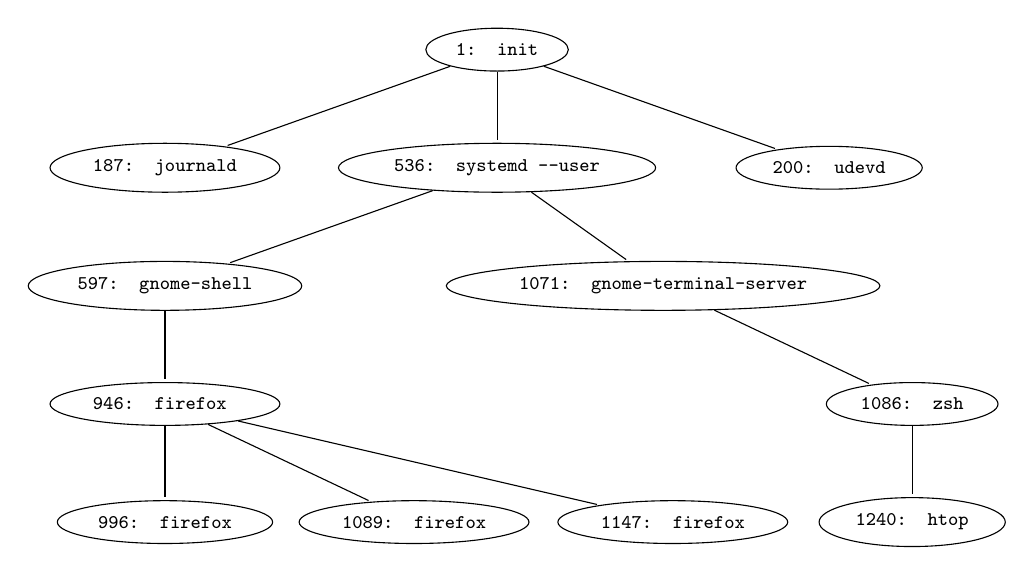
\begin{tikzpicture}[sibling distance=12em]
      \tikzstyle{every node}=[ellipse, draw, font=\scriptsize\ttfamily, align=center]
      \node {1: init}
        child { node {187: journald} }
        child { node {536: systemd --user}
          child { node [xshift=-6em] {597: gnome-shell}
            child { node { 946: firefox }
              child { node [xshift=12em] {996: firefox} }
              child { node [xshift=9em] {1089: firefox} }
              child { node [xshift=6.35em] {1147: firefox} }
            }
          }
          child { node {1071: gnome-terminal-server}
            child { node [xshift=9em] {1086: zsh}
              child { node {1240: htop}
              }
            }
          }
        }
        child { node {200: udevd} };
    \end{tikzpicture}
  \end{frame}

  \begin{frame}
    \frametitle{How You Can See Your Process Tree}

    Use \texttt{htop}

    \hspace{2em} \texttt{sudo pacman -S htop} to install on the virtual machine

    \vspace{2em}

    You can press \texttt{F5} to switch between tree and list view

    \vspace{2em}

    You may have to update all your packages first:

    \hspace{2em} \texttt{sudo pacman -Syu} (Reboot if your kernel updates)
  \end{frame}

  \begin{frame}
    \frametitle{The Parent Process is Responsible for Its Child}

    The operating sets the exit status when a process terminates (by calling exit)

    \hspace{2em} It can't remove its PCB yet

    \vspace{2em}

    The minimum acknowledgment the parent has to do is read the child's exit status

    \vspace{2em}

    There's two situations:
    \begin{enumerate}
      \item The child exits first (zombie process)
      \item The parent exits first (orphan process)
    \end{enumerate}
  \end{frame}

  \begin{frame}
    \frametitle{A Zombie Process Waits for Its Parent to Read Its Exit Status}

    The process is terminated, but it hasn't been acknowledged

    \vspace{2em}

    A process may have an error in it, where it never reads the child's exit status

    \vspace{2em}

    The operating can interrupt the parent process to tell it to acknowledge the child

    \hspace{2em} This is a basic form of IPC called a signal (which may be ignored)

    \vspace{4em}

    The operating system has to keep a zombie process until it's acknowledged

    \hspace{2em} If the parent ignores it, the zombie process needs to wait to
    be re-parented
  \end{frame}

  \begin{frame}
    \frametitle{An Orphan Process Needs a New Parent}

    The child process lost its parent process

    \hspace{2em} The child still needs a process to acknowledge its exit

    \vspace{2em}

    The operating system re-parents the child process to \texttt{init}

    \hspace{2em} The \texttt{init} process is now responsible to acknowledge the
                 child
  \end{frame}

  \begin{frame}
    \frametitle{The Operating System Creates and Runs Processes}

    The operating system has to:
    \begin{itemize}
      \item Loads a program, and create a process with context
      \item Maintain process control blocks, including state
      \item Switch between running processes using a context switch
      \item Unix kernels start an \texttt{init} process
      \item Unix processes have to maintain a parent and child relationship
    \end{itemize}
  \end{frame}
\end{document}
